\documentclass[12pt, oneside]{article}
\usepackage[letterpaper, margin=1in, headsep=0.5in]{geometry}
\usepackage[english]{babel}
\usepackage[utf8]{inputenc}
\usepackage{amsmath}
\usepackage{amsfonts}
\usepackage{amssymb}
\usepackage{tikz}
\usetikzlibrary{quotes, angles}
\usepackage{graphicx}
%\usepackage{pgfplots}
%\pgfplotsset{width=10cm,compat=1.9}
%\usepgfplotslibrary{statistics}
%\usepackage{pgfplotstable}
%\usepackage{tkz-fct}
%\usepackage{venndiagram}

\usepackage{fancyhdr}
\pagestyle{fancy}
\fancyhf{}
\rhead{\thepage \\Name: \hspace{1.5in}.\\}
\lhead{BECA / Dr. Huson / Geometry 10th Grade\\* Unit 1b: Introduction to Geometry}

\renewcommand{\headrulewidth}{0pt}

\begin{document}
\subsubsection*{Do Now 1b.1: Drawing angles}
  \vspace{0.5cm}
  \begin{enumerate}
    \item Absolute value: Find the value of $|180-120|+|60-90|$. \vspace{2cm}

    \item Identify two rays in the given plane.\\[0.25in]
      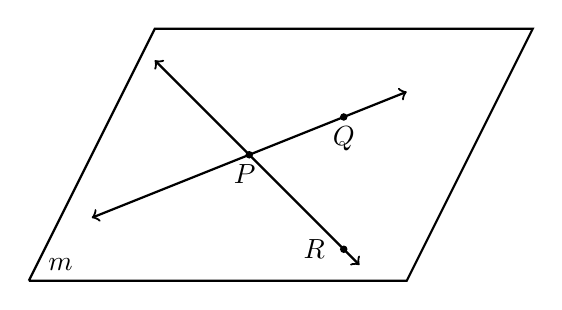
\begin{tikzpicture}[scale=0.8]
        \draw [thick](0,0) node[above right]{$\ m$} --(6,0)--(8,4)--(2,4)--(0,0);
        \draw [<->, thick] (1,1)--(6,3);
        \draw [fill] (3.5,2) circle [radius=0.05] node[below]{$P \ $};
        \draw [fill] (5,2.6) circle [radius=0.05] node[below]{$Q$};
        \draw [<->, thick] (2,3.5)--(5.25,.25);
        \draw [fill] (5,0.5) circle [radius=0.05] node[left]{$R \ $};
      \end{tikzpicture}
      \vspace{1cm}

    \item Given opposite rays $\overrightarrow{AB}$ and $\overrightarrow{AC}$, with $\overline{AB}=6$ cm. Draw a ray $\overrightarrow{AD}$ such that $m \angle BAD=60^\circ$ and $\overline{AD}=6$ cm.
    \vspace{7cm}
    \begin{center}
    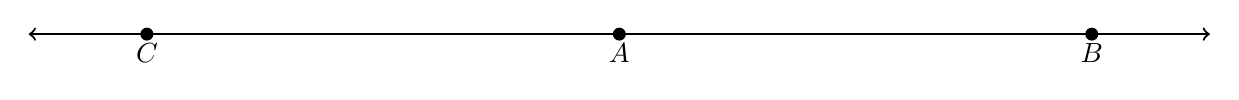
\begin{tikzpicture}[scale=1.5]
      \draw [->, thick] (0,0)--(-5,0);
      \draw [->, thick] (0,0)--(5,0);
      %\draw [->, thick] (0,0)--(-1.2,3);
      %\draw [fill] (-1,2.5) circle [radius=0.05] node[left ]{$B$};
      \draw [fill] (-4,0) circle [radius=0.05] node[below]{$C$};
      \draw [fill] (0,0) circle [radius=0.05] node[below]{$A$};
      \draw [fill] (4,0) circle [radius=0.05] node[below]{$B$};
    \end{tikzpicture}
    \end{center}

  \newpage
    \item Points that are all located on the same plane are $\rule{4cm}{0.15mm}$.

      \item Given collinear points $P, Q, R$ with $Q$ bisecting the line segment $\overline{PR}$. $PQ=x-2$ and $QR = \frac{1}{2} x+6$. Find the length of $\overline{PR}$.\\ \bigskip
      First label the drawing.
      \begin{flushright}
      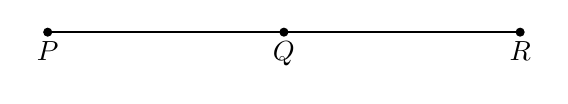
\begin{tikzpicture}
        \draw [-, thick] (0,0)--(6,0);
        \draw [fill] (0,0) circle [radius=0.05] node[below]{$P$};
        \draw [fill] (6,0) circle [radius=0.05] node[below]{$R$};
        \draw [fill] (3,0) circle [radius=0.05] node[below]{$Q$};
      \end{tikzpicture}
      \end{flushright}
      \vspace{1cm}
      \begin{enumerate}
        \item Write a geometric equation: \rule{4cm}{0.15mm} \hspace{1cm} \rule{4cm}{0.15mm}
        \vspace{.7cm}
        \item Substitute algebraic values: \rule{4cm}{0.15mm}
        \item Solve for $x$
        \vspace{4.5cm}
        %\begin{center} $x=$ \rule{1cm}{0.15mm} \end{center}
        \item Answer the question:
        \vspace{2.5cm}
        \item Check your answer
      \end{enumerate}


  \end{enumerate}

\end{document}
